% arara: xelatex
% arara: xelatex
% arara: xelatex


% options:
% thesis=B bachelor's thesis
% thesis=M master's thesis
% czech thesis in Czech language
% english thesis in English language
% hidelinks remove colour boxes around hyperlinks

\documentclass[thesis=B,english]{FITthesis}[2019/03/06]

%\usepackage[utf8]{inputenc} % LaTeX source encoded as UTF-8
% \usepackage[latin2]{inputenc} % LaTeX source encoded as ISO-8859-2
% \usepackage[cp1250]{inputenc} % LaTeX source encoded as Windows-1250

% \usepackage{subfig} %subfigures
\usepackage{amsmath} %advanced maths
% \usepackage{amssymb} %additional math symbols

\usepackage{dirtree} %directory tree visualisation
\usepackage[style=iso-numeric, maxcitenames=1, maxbibnames=1]{biblatex}

\addbibresource{bibliography.bib}

% % list of acronyms
% \usepackage[acronym,nonumberlist,toc,numberedsection=autolabel]{glossaries}
% \iflanguage{czech}{\renewcommand*{\acronymname}{Seznam pou{\v z}it{\' y}ch zkratek}}{}
% \makeglossaries

% % % % % % % % % % % % % % % % % % % % % % % % % % % % % % 
% EDIT THIS
% % % % % % % % % % % % % % % % % % % % % % % % % % % % % % 

\department{Department of Information Security}
\title{Timing side-channel attack on AES}
\authorGN{Adam} %author's given name/names
\authorFN{Zahumenský} %author's surname
\author{Adam Zahumenský} %author's name without academic degrees
\authorWithDegrees{Adam Zahumenský} %author's name with academic degrees
\supervisor{Ing. Jiří Buček, Ph.D.}
\acknowledgements{
	I thank my supervisor Jiří Buček for his time and ideas which helped me delve deeper into my discoveries.
	Furthermore, I thank all of my friends for their unending support when I needed it the most.
}
\abstractEN{
	This work demonstrates a timing side-channel attack on the AES-128 cipher using modern hardware.
    It provides software which leverages such attack to test a provided AES-128 implementation for vulnerability.
	The software is provided in a form suitable for use as an InfoSec laboratory assignment.
    Finally, it demonstrates that the latest OpenSSL release is under certain conditions still vulnerable to the attack.
}
\abstractCS{
	Tato práce demonstruje časový postranní útok na šifru AES-128 s využitím současného hardwaru.
	Jejím výsledkem je software, který takový útok využívá k odhalení zranitelnosti v poskytnuté implementaci AES-128.
	Software je vyvinutý s účelem využití ve výuce počítačové bezpečnosti jako laboratorní úkol.
	Práce nakonec demonstruje tuto zranitelnost za určitých podmínek v nejnovější verzi OpenSSL.
}
\placeForDeclarationOfAuthenticity{Prague}
\keywordsCS{AES, postranní útok, časový útok, informační bezpečnost}
\keywordsEN{AES, side-channel attack, timing attack, information security}
\declarationOfAuthenticityOption{2} %select as appropriate, according to the desired license (integer 1-6)
% \website{http://site.example/thesis} %optional thesis URL


\begin{document}

% \newacronym{CVUT}{{\v C}VUT}{{\v C}esk{\' e} vysok{\' e} u{\v c}en{\' i} technick{\' e} v Praze}
% \newacronym{FIT}{FIT}{Fakulta informa{\v c}n{\' i}ch technologi{\' i}}

\setsecnumdepth{part}
\chapter{Introduction}

AES (Advanced Encryption Standard) is one of today's most widely used symmetric ciphers.
It features sufficient performance for real-time data encryption, being featured prominently in disk encryption and secure messaging.
In this work, I limit my scope to AES-128, an AES variant using a 128-bit key.

The cipher is still considered safe for use with sensitive data. 
Several cryptographic attacks on the cipher exist with the latest one only about 4x faster than a brute force attack \cite{bogdanov2011biclique}.
Given the $2^{128}$ operations a brute-force attack would require, an attack with such speedup is still completely unfeasible on today's hardware.

Despite the cipher's resistance to cryptographic attacks, side-channel attacks may be used to break specific implementations.
Side-channel attacks target implementation flaws and require additional information about the encryption to break the key.
In this thesis, the targeted side channel is encryption time.

To protect encryption algorithms from leaking side channels, manufacturers tend to include cryptographic support in hardware, a move proven to be very efficient.
Hardware implementations are faster and more secure as the cryptographic operations are moved away from RAM and caches into dedicated hardware and registers.
However, hardware support is not omnipresent and software implementations of AES are still critical for systems without such support.

This work aims to present a complete software package able to test any AES-128 implementation for timing side-channel vulnerability.
It is provided in the form of a laboratory assignment for students of hardware security at FIT CTU.
Besides testing self-written AES implementations I also test the latest OpenSSL build and document my findings.


\setsecnumdepth{all}
\chapter{AES-128 cipher}

\section{Basic principles}
AES-128 is a symmetric block cipher using the substitution-permutation network design.
It accepts a 16-byte key $k$, a 16-byte input block $n$ and outputs a scrambled 16-byte data block.

A symmetric cipher uses the same key for both encryption and decryption. As such, obtaining the key enables an attacker to both read and write data.
On the other hand, it simplifies implementations, leading to cheaper dedicated hardware and lower hardware requirements.

A block cipher encrypts data per blocks of fixed size. In the case of AES-128, the block size is 128 bits. 
Data larger than the block size are then sliced and padded to 16-byte blocks which are then sequentially encrypted and chained using a specific operation mode.
One can safely ignore the various cipher operation modes by limiting themselves to repeated encryptions of a single block.

For simplicity, I shall omit AES decryption since this work only uses encryption to gather data.

\subsection{Encryption}
AES-128 works with an internal 16-byte state $s$ initialized to $n \oplus k$ where $\oplus$ denotes the bitwise XOR. It is represented as a 4x4 2D matrix.
The key is first expanded to 10 16-byte round keys $rk$, one for each round, using the Rijndael key schedule \cite{FIPS}[section 5.2].
The state is then scrambled in 10 rounds consisting of four steps in this order: \textit{SubBytes}, \textit{ShiftRows}, \textit{MixColumns} and \textit{AddRoundKey}.
The 10th round omits the \textit{MixColumns} step.
\pagebreak

\textit{AddRoundKey} mixes the current round key $rk_i$ into the state: $s' = s \oplus rk_i$.\vspace{0.1cm}

\textit{SubBytes} uses a fixed 256-byte substitution table $S$ called an S-box, commonly implemented as a plain array.
The state is then substituted byte for byte using the S-box: $s' = S[s]$.\vspace{0.1cm}

\textit{ShiftRows} rotates the last three rows to the right: second row by 1, third row by 2 and fourth row by 3.\vspace{0.1cm}

\textit{MixColumns} scrambles each column of the state by the following invertible linear transformation:
$$
\begin{bmatrix}
	s'_{0,j} \\ s'_{1,j} \\ s'_{2,j} \\ s'_{3,j}
\end{bmatrix} = \begin{bmatrix}
	02 & 03 & 01 & 01 \\
	01 & 02 & 03 & 01 \\
	01 & 01 & 02 & 03 \\
	03 & 01 & 01 & 02
\end{bmatrix} \begin{bmatrix}
	s_{0,j} \\ s_{1,j} \\ s_{2,j} \\ s_{3,j}
\end{bmatrix}
$$
All bytes above represent polynomials over GF($2^8$) of order $x^7$. All additions are bitwise XOR and multiplications are done modulo $x^8+x^4+x^3+x+1$.

\section{T-box optimization}
A well-known optimization of the above procedure is to combine the three mentioned steps into one large tabular substitution using four 1024-bit tables known as T-boxes.
The following definitions are sourced from \cite{TBOX} and \cite{bernstein2005cache}.
Each T-box can be viewed as 256 4-byte values defined as follows:
$$
T_0[j] = \begin{bmatrix} 02.S[j] \\ S[j] \\ S[j] \\ 03.S[j] \end{bmatrix}
T_1[j] = \begin{bmatrix} 03.S[j] \\ 02.S[j] \\ S[j] \\ S[j] \end{bmatrix}
T_2[j] = \begin{bmatrix} S[j] \\ 03.S[j] \\ 02.S[j] \\ S[j] \end{bmatrix}
T_3[j] = \begin{bmatrix} S[j] \\ S[j] \\ 03.S[j] \\ 02.S[j] \end{bmatrix}
$$
Bytes here are again considered polynomials over GF($2^8$) as above.
The first nine rounds can then be simplified to the following transformation using the round key $rk_i$.
\begin{equation}
\label{eq:tboxround}
s' = \begin{bmatrix}
	T_0[s_{0,0}] \oplus T_1[s_{1,1}] \oplus T_2[s_{2,2}] \oplus T_3[s_{3,3}] \oplus rk_i[0] \\
	T_0[s_{1,0}] \oplus T_1[s_{2,1}] \oplus T_2[s_{3,2}] \oplus T_3[s_{0,3}] \oplus rk_i[1] \\
	T_0[s_{2,0}] \oplus T_1[s_{3,1}] \oplus T_2[s_{0,2}] \oplus T_3[s_{1,3}] \oplus rk_i[2] \\
	T_0[s_{3,0}] \oplus T_1[s_{0,1}] \oplus T_2[s_{1,2}] \oplus T_3[s_{2,3}] \oplus rk_i[3]
\end{bmatrix}
\end{equation}
\textit{AddRoundKey} is already included in this transformation, interpreting $rk_i$ as a four 4-byte values.
The last round is usually not optimized and simply consists of \textit{SubBytes}, \textit{ShiftRows} and \textit{AddRoundKey}.

\chapter{Timing attacks on AES}

\section{Introducing timing side-channel attacks}
Side-channel attacks take a different approach from traditional cryptographic attacks.
Instead of attacking the cipher mechanism head-on they target weaknesses of specific implementations.
Vulnerable implementations may leak information such as electromagnetic waves, power consumption or timing.

This work focuses on the timing side channel, the time an implementation takes to process data.
In the case of AES, the simplest timing target is the time taken to encrypt a single block of data.

The only way to make a software AES implementation resistant to leaking timing data is to make it run in constant time.
\textit{``It is extremely difficult to write constant-time high-speed AES software for common general-purpose computers."}, Bernstein stated in \cite[Abstract]{bernstein2005cache}.
The performance penalty imposed on constant-time AES software is unacceptable for generic use in demanding applications like disk encryption.

Hardware-supported encryption has the benefit of not using RAM and caches, cutting off access from prying eyes.
Moreover, it offers significant performance improvements as lookup tables are hard-wired into the hardware.
By extension, this also has the potential to make timing attacks more difficult as caches are not used at all.

\subsection{Exploiting caches}
Every AES implementation needs one or more lookup tables for the substitution steps.
In the case of T-box optimized implementations, there is up to 4~kB of lookup data to store in memory.

With recent L1 caches easily hitting hundreds of kB in size, it is expected that the tables will be cached on all levels of the cache hierarchy.
As Kocher wrote in 1996, \textit{``RAM cache hits can produce timing characteristics''}\cite[section 11]{kocher1996}.
If certain lines from the lookup tables get kicked out of cache and are accessed later, the miss penalty can be detected.
These penalties may help an attack if they are well correlated with controlled variables such as the input block or a known key.

\section{Bernstein's attack}
Bernstein aimed his timing attack at the T-box optimized software implementation of AES-128 in OpenSSL and demonstrated its usability over the network.
He based his attack on the following assumption:
\textit{``it is extremely difficult to load an array entry in time that does not depend on the entry’s index''}\cite{bernstein2005cache}.

The first round of T-box optimized AES-128 accepts $n \oplus k$ as the input state.
Therefore the time of the first T-box lookup should be dependent on bytes of both $k$ and $n$.
As all 16 bytes of $s$ are used as indices in def. \ref{eq:tboxround}, all bytes of the key could be correlated with timing using the first round alone.

\subsection{Design}
The attack targets a network-accessible victim machine and is split into client and server roles.

The client sends packets of set size to the server which performs encryption using its own secret key $k$.
Bernstein demonstrated his results with 400, 600, and 800-byte packets.
Each packet contains random data, and the server only encrypts the first 16 bytes as $n$.
It then echoes back the encrypted block followed by encryption time and the unchanged remainder of the packet.

As a result, each random packet sent equals one encryption by the server plus some extra ``work", in this case, the echoing of data back to the client.
Bernstein modeled the attack this way to simulate a real server which accepts some work request alongside with additional data.
As the server sends back the encryption time, there is no need to gather extra measurements to amount for variable network delays.

The client then tallies the responses for each byte of the cleartext $n$.
The output data of the client has the form of timing statistics for each $n$ byte $[0,15]$ and its value $[0,255]$.

The client outputs are later fed to a correlating program that tries to identify possible candidates of $k$.
In the end, a brute-force program tests these candidates in a loop and tries to break $k$.

\subsection{Principle}
\label{section:bernstein_impl}
In the first stage, the attacker uses their own machine with an identical CPU to the victim's machine.
The key $k_1$ is known in this case and defaults to zero in Bernstein's implementation, hence $n = k_1 \oplus n$.
The attacker then runs the server on this machine and collects timing data for random blocks $n_1$ using $k_1$.

The second stage involves the server running on the victim's machine and its secret key $k_2$. Data collection for random blocks $n_2$ is the same as above.

With both datasets collected, as both machines use the same CPU and implementation, it is safe to assume that if a correlation exists between $n_1 \oplus k_1$ and encryption time,
that correlation\footnote{Bernstein used plain covariance instead} is identical for $n_2 \oplus k_2$.

The attacker then goes over all 16 bytes of $k_2$ and searches for such a value of $c$ which would cause the two datasets, $k_1[i] \oplus n_1[i]$ and $c \oplus n_2[i]$, to correlate the best.
These values of $c$ then become the byte candidates for $k_2[i]$.

\subsection{Results}
Bernstein successfully cracked a whole AES-128 key using two machines running Intel Pentium III, now a very old CPU with only two levels of caches.
A single run of the attack didn't break every byte but multiple runs with different packet sizes cracked different bytes, eventually revealing enough of the key to run a brute-force attack.

\section{Further work}
Wei Liu et al. tested Bernstein's attack on an Intel Atom N2800, Intel Xeon E5410 and Intel Core i5 with the Atom showing very limited vulnerability,
reducing the key space from $2^{128}$ to $2^{112}$ \cite{WEI}.
The attack was completely unsuccessful on the latter CPUs but considering the minor keyspace reduction, the Atom was also found practically resistant.

C Ashokkumar et al. used a different type of attack on an Intel Core i3-2100 and Intel Core i7-3770 \cite{ASHOKKUMAR}.
They successfully used the cache-based Prime+Probe and Flush+Reload techniques to break an AES-128 key.
In this case, the target implementation was not optimized using the T-boxes and instead used the traditional 256-byte S-box.
Their work proves that the software implementations of AES are vulnerable to cache attacks even on recent processors.
Similar results were achieved by Liwei Zhang et al. who targeted an Intel Core i5 CPU and again used cache-based attacks to extract the key \cite{ZHANG}.

I found no further successful endeavors using Bernstein's original attack principle.

\chapter{Designing the attack}
Before designing my own attack I tested Bernstein's original attack on my Intel Core i5-6300HQ machine running Linux 5.0.
Based on my observations I then designed a modified attack better suiting its intended use.

\section{Testing Bernstein's attack}
Bernstein included the whole source of his attack in \cite{bernstein2005cache}, allowing me to build it myself.
I built the server against my system-wide OpenSSL version 1.1.1b, the latest stable release today.
The simplest way to test it was to run both stages of the attack on the same machine.

Running the attack in its original form brought fruitless results, not detecting any of the key's bytes.

After a closer inspection of the client code, I found a hard-coded tail clip cutoff for timings.
This value was apparently tuned for a Pentium III, defined at 10 000 ticks per single block encryption.
Observing the data dumped by the client program, I noticed the threshold was almost 30x higher than the average encryption time.
After tweaking the threshold to 5x the average, the attack cracked several bits of the key.
These are shown in table \ref{tbl:bernstein_result} as the number of candidates for each byte of $k$.

Bernstein uses the x86 RDTSC instruction, which reads the timestamp counter register.
Therefore context switches have a deeply negative impact on the precision of measurement.

\begin{table}
	\centering
	\begin{tabular}{c|c c c c c c c c}
		$i$ & 0 & 1 & 2 & 3 & 4 & 5 & 6 & 7 \\
		candidates & 32 & 80 & 256 & 256 & 113 & 69 & 256 & 256 \\
		\hline
		$i$ & 8 & 9 & 10 & 11 & 12 & 13 & 14 & 15 \\
		candidates & 241 & 96 & 256 & 256 & 228 & 94 & 256 & 256
	\end{tabular}
	\caption{Number of candidates for bytes of $k$ detected by Bernstein's attack}
	\label{tbl:bernstein_result}
\end{table}

\section{Defining improvements}
\label{section:designlist}
The partial success of the modified Bernstein's software convinced me to build my work on top of it using the same core principle but bringing these modifications:
\begin{enumerate}
	\item The network aspect including variable-size packets is dropped and all the work happens on a single machine
	\item It compiles and runs under Linux and Microsoft Windows 10, considering both operating systems are installed on the machines in the InfoSec laboratory at FIT CTU
	\item A variable number of ``study'' keys are observed and their timings correlated to the target key's dataset
	\item The cutoff threshold for discarding excessive timings is determined at runtime to account for differently performant machines
	\item The tested AES implementation is chosen by the user
	\item Output data is visualized and sorted to facilitate manual analysis
	\item Pearson's correlation coefficient is used to define correlations
	\item Caches may be optionally purged before each encryption to measure their impact on the attack
	\item Data visualizer is added for convenience
	\item The attack is automated and configurable for various use cases
\end{enumerate}

\chapter{Implementation}
The final software is split into two units: an encryption core (further referred to as the ``core'') written in C and an analytic wrapper (further on simply ``wrapper'') written in Python.
Additionally, a small 128-bit key generator written in Python is provided for convenience.
This separation of tasks let me delegate visualization and data analysis to the robust Numpy and Matplotlib Python libraries while retaining maximum performance for the encryption itself.

The building of the core is handled by GNU Make on Linux and NMAKE (Microsoft Program Maintenance Utility) on Windows.
The makefiles let the user configure options such as OpenSSL location or implementation selection, and provide targets for running tasks.

\section{Encryption core}
The core fulfills two roles: gathering correlation data and brute-forcing the key.
The current role is chosen based on the presence (or lack thereof) of a brute-force candidate file, \verb'bf.dat'.

\subsection{Encrypting blocks}
Data blocks to encrypt are generated pseudo-randomly.
The user may choose between the standard C \verb'rand', or OpenSSL's \verb'RAND_bytes' PRNGs but \verb'rand' seems to suffice and is faster.
If encryption time exceeds the cutoff threshold, it is performed again until the criterion is met.

Testing of custom implementations is enabled by the supplied \verb'aes.h' header which must first be implemented.
This entails three functions for initialization, key expansion, and encryption.
The custom implementation is then added to the makefile via a provided variable.

\subsection{Gathering correlation data}
\label{section:gathering_corr_data}
The target key $k$ may be provided in a file or randomly generated.
The number $N_k$ of test keys to correlate against $k$ and the number $N_b$ of $n$ to encrypt and measure per key is chosen at compile time.

Before actual data gathering takes place $N_b$ block encryptions are measured without a threshold and total time is measured using a monotonic timer to calculate the average encryption time.
The cutoff threshold is then defined as a fixed multiple of this average and the rate of encryption per second is dumped for use by the wrapper.

$N_b$ block encryptions are then measured for $k$ and $N_k$ randomly generated test keys.
The correlation is calculated for each test key as described in section \ref{section:bernstein_impl} and summed per $k$ byte candidate.
As Pearson's correlation coefficient returns values from $[-1, 1]$, the resulting correlation values for each $k$ byte candidate lie in $[-N_k, N_k]$.
These are sorted per byte and dumped to \verb'corr.txt' for analysis by the wrapper.

\subsection{Brute force attack}
When a \verb'bf.dat' file exists, the core tries to break $k$ by brute force. The file contains candidates for each $k$ byte sorted by relevance.
It is assumed that the more candidates exist for a given byte, the less likely the correct value is at the front.
Therefore the bytes with the least candidates are rotated last while trying.
Every candidate key encrypts a zero block and the result is compared to the scrambled zero produced by $k$.

\section{Analytic wrapper}
\label{section:wrapper}
One of this python script's roles is visualizing the correlations for all 256 values of the 16 bytes of $k$ using matplotlib, producing 16 graphs as shown in Appendix \ref{appendix:measurements}.
The other is automating the process of data collection and analysis.

\subsection{Peak detection}
After invoking the core and reading its correlation outputs, the wrapper attempts to detect significant peaks in the correlation values per $k$ byte.
As testing has shown in section \ref{section:testing}, the bytes of $k$ which leak data sport significant visually discernible peaks.

First, the mean absolute deviation is calculated for the data trimmed off 32 highest and lowest values. For explanation on this number see section \ref{section:bits}.
Peak values are then defined as all values exceeding a fixed multiple of this deviation.
The method was chosen based on the observation of peak sizes which rarely exceed 32 bytes.
Naturally, this method is not exact and tends to produce occasional false positives depending on the dataset.

\subsection{Byte pools}
Peak values gathered as $k$ byte candidates are called a ``byte pool''.
For reasons detailed in section \ref{section:aslr}, the wrapper generates new data in a loop, adding the received correlations to the summary candidate dataset $C$.
Once new data is gathered by the core, the wrapper performs peak detection, and the resulting candidates are intersected with the existing candidates in $C$.
This results in a gradual reduction of pool sizes as more data is acquired. If a pool shrinks to zero, it is removed.
Moreover, this method provides self-healing of false positives as the pools containing them are likely to be removed eventually, hinting false positives to the user.

All byte candidates in $C$ and the pools are kept sorted by their sum of measured correlations.
The wrapper uses encryption rate provided by the core to estimate the worst time a brute-force attack would take.
When the time drops below a set threshold, the wrapper dumps the sorted candidates to \verb'bf.dat'. For bytes associated with a pool, only the pool members are dumped.
The core is then invoked to try breaking the key.

\subsection{Checkpoints}
To facilitate analysis, the wrapper backs up the received correlations after each collection and creates a checkpoint by dumping the current pools and sorted $C$ to disk.
The dumped $C$ can be analyzed manually or visualized directly using the wrapper. Both give the user a detailed overview of the attack's progression.

If the checkpoints are present, the wrapper loads them automatically at the start, effectively making the attack interruptible.

\chapter{Testing} 
\label{section:testing}
To document all possible factors affecting the attack, I used my own T-box optimized implementation, which had already proven itself somewhat vulnerable to Bernstein's original attack.
Unless stated otherwise, the tests were run on an Intel Core i5-6300HQ machine running Linux and the used params are $N_k = 1$ and $N_b = 2^{23}$.

\subsection{ASLR}
\label{section:aslr}
ASLR (address space layout randomization) is a feature of modern operating systems, including Linux and Windows, where the address layout of a new process is randomized.
This is done by adding random offsets to the binary's sections.
Under Linux, tweaking ASLR is done by setting the \verb'kernel.randomize_va_space' kernel parameter to 0, 1, or 2.
According to \cite{kernelASLR}, the setting of 2 only adds heap randomization to the presets of 1. 0 turns ASLR off completely.

Multiple runs of the attack using the same $k$ would sometimes leak different bits of the key.
A quick experiment with turning off ASLR entirely caused the attack to always leak information about the same bytes.
T-boxes in both mine and OpenSSL's fallback implementation are global constants placed in the (read-only) data segment.
There should thus be no difference between the ASLR settings of 1 and 2.
Table \ref{tbl:aslr} shows the impact of ASLR on the attack and confirms that assumption.
It also shows that disabled ASLR limits the attack to the bytes leaking in a single core run, making repeated core runs pointless.

\begin{table}
	\centering
	\begin{tabular}{c|c|c|c}
		Runs & ASLR 0 & ASLR 1 & ASLR 2 \\
		 1 & 3 & 4 & 3 \\
		 5 & 3 & 10 & 9 \\
		 10 & 3 & 13 & 12
	\end{tabular}
	\caption{Number of leaking bytes of $k$ over time for $N_k = 1$}
	\label{tbl:aslr}
\end{table}

Attempting to raise $N_k$ to yield more data from a single run proved fruitless. The individual key correlations apparently leak identical data.
While this makes the correlation peaks more pronounced and easier to detect, it doesn't let one crack more bytes of $k$.
Setting $N_k = 20$ and re-running the same benchmark yielded exactly the same results, only the peaks were significantly amplified.

\subsection{T-boxes and memory layout}
\label{section:memlayout}
Observing the behavior of both my T-box implementation and OpenSSL's fallback implementation (discussed in section \ref{section:testing_openssl}), I noticed the leaked bytes followed a pattern.
A vast majority of vulnerable bytes are offset from each other by a multiple of 4:
\begin{align}
	I_{max} &= \{i, i+4, i+8, i+12\}, i \in \{0,1,2,3\} \nonumber \\
	I_k &\subseteq I_{max}
	\label{eq:fourhex}
\end{align}
where $I_k$ denotes the indices of all bytes of $k$ which leak data in a given run. $I_{max}$ is a bounding set for $I_k$.

The occurrence of measurements where $I_k$ contains additional vulnerable byte indices is very rare and if it happens, the extra bytes tend to leak a low number of bits.
I measured data for 50 random keys and categorized them by their bounding $I_{max}$ in table \ref{tbl:pool_tally} which shows this behavior.

\begin{table}
	\centering
	\begin{tabular}{c|c|c|c|c|c}
		$I_{max}$ & \{0, 4, 8, 12\} & \{1, 5, 9, 13\} & \{2, 6, 10, 14\} & \{3, 7, 11, 15\} & Other \\
		Runs & 16 & 13 & 11 & 10 & 0
	\end{tabular}
	\caption{50 runs tallied by their $I_{max}$}
	\label{tbl:pool_tally}
\end{table}

\subsubsection{Critical indices}
\label{section:crit_indices}
It is obvious that the spacing of $I_{max}$ is not random. The definition of a T-box round in fig. \ref{eq:tboxround} shows that the T-box $T_i$ is indexed with bytes from the $i$-th column of $s$, ie. every 4th byte of $s$.
As the first round of AES initializes $s$ to $n \oplus k$, by def. \ref{eq:fourhex} all bytes $k[i], i \in I_k$ are used in indexing a single T-box in the first round. 

In other words, the leaks seem to be linked to a single T-box which is time-sensitive to certain indices $i_c$.

Let's define the bytes of $n$ for each vulnerable index $i \in I_k$ which take an unusually long time to encrypt as $n[i]_{max}$. Then
$$
i_c = \{ n_c[i] \oplus k[i] \mid n_c \in n[i]_{max}, i \in I_k \}
$$

As all vulnerable bytes of $s$ are used with the same T-box, the values of $i_c$ should stay the same for all $i \in I_k$.

This supports Bernstein's statement about time-dependent array indexing.
I tried to detect $i_c$ values with disabled ASLR to prevent the tables from changing addresses.
The measurements in table \ref{tbl:tbox_indices} show that the values of $i_c$ indeed remain constant across indices in $I_k$ when using various keys $k$ with a constant memory layout.

As $i_c$ holds a single value of $\text{2c}_{16}$, the vulnerable bytes of $k$ in the used configuration may be defined as
$$
k[i] = \text{2c}_{16} \oplus n[i]_{max}[0], i \in I_k
$$

\begin{table}
	\centering
	\begin{tabular}{c|c|c|c}
		$I_k$ & $k[i], i \in I_k$ (hex) & $n[i]_{max}, i \in I_k$ (hex) & $i_c$ (hex) \\
		\{1, 9, 13\} & \{8e, a4, 20\} & \{\{a2\}, \{88\}, \{0c\}\} & \{2c\} \\
		\{1, 9, 13\} & \{1e, 08, df\} & \{\{32\}, \{24\}, \{f3\}\} & \{2c\} \\
		\{1, 9, 13\} & \{e7, da, bd\} & \{\{cb\}, \{f6\}, \{91\}\} & \{2c\} \\
		\{1, 9, 13\} & \{5a, 77, 1e\} & \{\{76\}, \{5b\}, \{32\}\} & \{2c\} \\
	\end{tabular}
	\caption{Values of $i_c$ taken for 4 random keys. $T_0$ base offset: $\text{8f60}_{16}$}
	\label{tbl:tbox_indices}
\end{table}

Similar results were obtained using OpenSSL's \verb'aes_core.c' implementation discussed in section \ref{section:testing_openssl} but with a different (yet also single) value of $i_c$, likely caused by a different memory layout and implementation details.
Enabling ASLR or otherwise changing the T-box addresses in memory had the expected effect of changing $i_c$ and sometimes also changing $I_k$.

These observations showed that a single T-box is responsible for the timing leaks and that the critical indices $i_c$ may be detected by testing with known keys.

\subsection{Leaking bits}
\label{section:bits}
Most core runs do not leak all 8 bits of a vulnerable key byte. Instead, they usually leak at least 3 bits, yielding candidate pools capped at 32 bytes.
This observation led me to design the 32-byte symmetric cutoff used in peak detection by the wrapper.

The bytes which leak less than 8 bits have a strong tendency to leak the highest bits first, creating a contiguous interval of candidates (see table \ref{tbl:leaking_bits} and fig. \ref{fig:limited_corr_byte}).
This means the values of $i_c$ also form a contiguous interval of indices of a T-box which is associated with high load times.

\subsubsection*{Graph note}
Starting with fig. \ref{fig:perfect_corr_byte} I present graphs plotting the total correlation values for all possible values of a $k$ byte.
The red dotted lines denote the maximum, not the actual value of $k[i]$.

\begin{figure}[h]
	\centering
	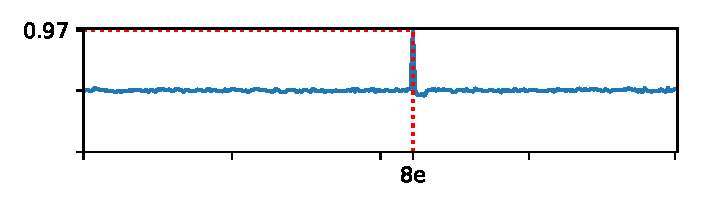
\includegraphics{superstrong_key_8e.pdf}
	\caption{A full-byte leak of $k[1] = \text{8e}_{16}$}
	\label{fig:perfect_corr_byte}
\end{figure}

\begin{figure}
	\centering
	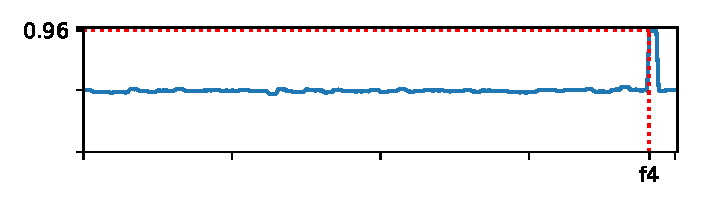
\includegraphics{broad_pool_example.pdf}
	\caption{A 6-bit leak of $k[0] = \text{f5}_{16}$}
	\label{fig:limited_corr_byte}
\end{figure}

\begin{table}
	\centering
	\begin{tabular}{c|c|c}
		$i \in I_k$ & Candidates (hex) & Bits leaked \\
		0 & 1d 1e 1c 1f & 6 \\
		4 & 51 52 50 53 & 6 \\
		8 & 24 26 27 20 25 22 21 23 & 3 \\
		12 & 70 & 8
	\end{tabular}
	
	\caption{Key candidates after a single core run}
	\label{tbl:leaking_bits}
\end{table}

\subsection{Connection with caches}
The correlation between memory layout and leaking bytes suggests that cache penalties are causing the timing spikes.
If a certain index of a T-box caused consistent cache misses, the resulting miss penalties could add up to a statistically significant timing spike.

To try and confirm the hypothesis, I tried purging all levels of cache before every encryption.
This would ensure the first round couldn't make use of cached T-boxes.

Doing this didn't stop the attack but made it slower and more difficult. 
Figure \ref{fig:cache_off_k4} shows that secret data is still at least partially leaking.

OpenSSL's \verb'aes_x86core.c' file contains a prefetch function for prefetching the last T-box (reading the whole T-box and caching it in the process).
I tried using the same function in my implementation of T-box AES, but it didn't stop the attack no matter which T-boxes I tried to prefetch.

I was unable to get conclusive data on what exact role caches play in the attack, but it seems the role is supportive.
This could be an interesting topic for future research.

\begin{figure}
	\centering
	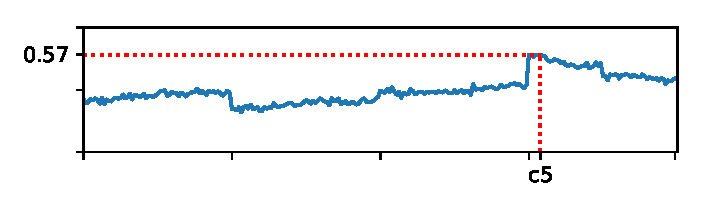
\includegraphics{caches_on_key_3e.pdf}
	\caption{A 3-bit leak of $k[0] = \text{c0}_{16}$ using purged caches}
	\label{fig:cache_off_k4}
\end{figure}

\section{The importance of cutoffs}
Disabling the cutoff threshold for encryption time stops the attack. The same behavior made Bernstein's implementation non-functional when the threshold was set too high.
Setting the cutoff too high or low makes the output very noise or very flat, respectively, both leading to failure.
See Appendix \ref{appendix:measurements} for an example with threshold cutoff turned off.

\section{Testing custom implementations}
I have three implementations I could test with the attack: a naive one, a T-box optimized one (the testing default), and one using Intel-specific AES-NI instructions \cite{IntelAESNI}.
The T-box implementation is vulnerable as it is the original target for this attack.

\subsection{Testing a naive implementation}
Since the naive implementation only uses a single 256-byte S-box table for lookup, there is a lower probability that it will leak timing data the same way.
Running the test with default options showed no results, so I set the configuration to $N_k = 25$, $N_b = 2^{25}$ and still got no apparent leak patterns (fig. \ref{fig:sbox_noleak}).
The output is extremely noisy, and there are no outstanding peaks.
I conclude the implementation as resistant, although such implementations are not usually found in production.

\begin{figure}
	\centering
	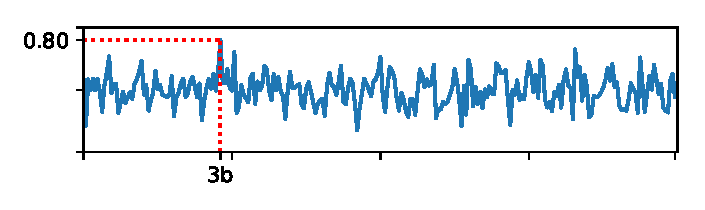
\includegraphics{sbox_example.pdf}
	\caption{Naive implementation is resistant ($k[0] = \text{4f}_{16}$)}
	\label{fig:sbox_noleak}
\end{figure}

\subsection{Testing an AES-NI implementation}
These instructions are using hardware-assisted encryption, hence cache and RAM access times cannot help with the attack.
Tweaking parameters to $N_k = 10, N_b = 2^{30}$ didn't help (fig. \ref{fig:aesni_noleak}).
The implementation is resistant.

\begin{figure}
	\centering
	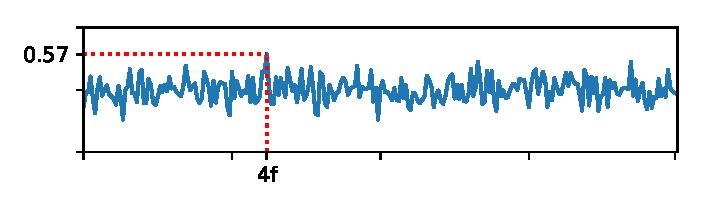
\includegraphics{ni_example.pdf}
	\caption{AES-NI implementation is resistant ($k[0] = \text{96}_{16}$)}
	\label{fig:aesni_noleak}
\end{figure}

\section{Testing OpenSSL implementations}
\label{section:testing_openssl}
OpenSSL compiles with hardware encryption support enabled by default. The project includes assembly definitions for various CPU architectures including AES-NI support.
Testing my system build of OpenSSL as well as OpenSSL built from source using the default configuration, I found no leaking bits, yielding noisy and empty results similar to fig. \ref{fig:aesni_noleak}.
I tested the default build on two machines: the default Core i5-6300HQ machine which supports AES-NI and a Core 2 Duo powered Linux machine which does not but it supports SSE3 instructions.
Neither of them leaked secret data.

OpenSSL does have a software implementation in the \verb'aes_core.c' file which is T-box optimized.
This implementation is only used as a fallback when the CPU does not support any of the more specific implementations or when the \textit{no-asm} option is used.
This explains why the default build on the Core 2 Duo machine stayed resistant despite lacking AES-NI support. It used an x86-specific constant-time SSE3 implementation instead.

Today finding a machine incapable of using any of the provided specific implementations is difficult.
Therefore I compiled OpenSSL with the \textit{no-asm} option and found it vulnerable similar to my T-box implementation (fig. \ref{fig:openssl_noasm_singlebyte}).
Very similar results were obtained using Windows 10 on an i5-8600K machine.

Testing the \textit{no-asm} build on the Core 2 Duo (fig. \ref{fig:openssl_noasm_coreduo_singlebyte}) yielded some very interesting results where multiple bytes leaked 64 candidates regularly split into quartets.
This hints at multiple evenly spaced critical indices, possibly due to the Core 2 Duo's smaller caches. See Appendix \ref{appendix:measurements} for an additional measurement showing this behavior.

\begin{figure}
	\centering
	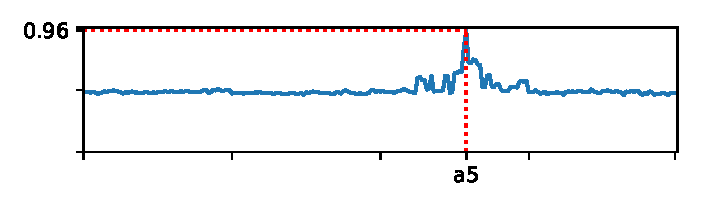
\includegraphics{openssl_noasm_laptop_byte.pdf}
	\caption{OpenSSL \textit{no-asm} implementation is vulnerable ($k[8] = \text{a5}_{16}$)}
	\label{fig:openssl_noasm_singlebyte}
\end{figure}

\begin{figure}
	\centering
	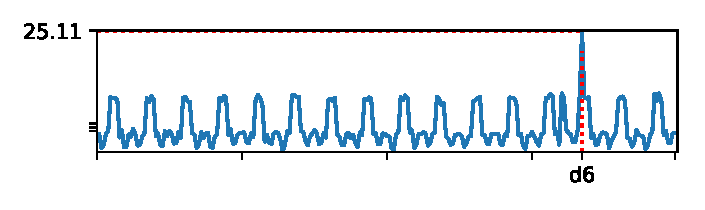
\includegraphics{openssl_noasm_core2duo_byte.pdf}
	\caption{OpenSSL \textit{no-asm} implementation on Core 2 Duo ($k[11] = \text{d6}_{16}$)}
	\label{fig:openssl_noasm_coreduo_singlebyte}
\end{figure}

\section{Testing on Windows and other machines}
Using the attack on Windows is possible. See Appendix \ref{appendix:measurements} for an example of a moderately leaked key.
However, I noticed that the attack is weaker on Windows, revealing data more slowly and having more false positives in the pools.
Nevertheless, the attack still works and leaks secret data.

\chapter{Laboratory assignment}
The intended use of this software is a laboratory assignment at the hardware security course at FIT CTU.
The course leads students to develop several implementations of AES-128 of ever-increasing performance.

I prepared guidelines for a possible assignment that would lead the students through understanding this attack's principle, testing their implementations and possibly testing OpenSSL on their machines.
The guidelines along with a guide to building and using the software are present in \verb'README.md'.
The attack is hardware and OS dependent, so students will get the chance to compare the attack's performance on various machines, including the provided lab PCs.

The first step is to introduce the students to the concept of timing attacks in general, and this specific attack.
To achieve this, I removed three topical portions of the core's code, prompting students to fill them in.
The portions are: tallying encryption times, calculating mean encryption times per each key byte, and correlating two datasets as detailed in section \ref{section:gathering_corr_data}.

The second step involves implementing the \verb'aes.h' header for all of the student's currently finished implementations of AES-128 and testing them for vulnerability.
This should give the students a comparison between the hardware-accelerated and immune AES-NI implementation and the software-optimized yet vulnerable T-box implementation.

The final step may consist of testing the attack on OpenSSL and comparing the vulnerability of its fallback implementation to the students' own.
This step is mostly informative but could be interesting for curious students.

In the end, more parts of the core may become fill-ins and the final form of the laboratory exercise will be subject to personal discussions with the course's teachers.

\setsecnumdepth{part}

\chapter{Conclusion}
The main goal of the thesis was to demonstrate the feasibility of a timing side-channel attack on the AES-128 cipher using modern processors, and it was successfully fulfilled.
I expanded on an already existing attack and produced software exploiting a timing side-channel vulnerability in a provided AES-128 implementation.
The software is, in some cases, capable of extracting the whole 128-bit key.

Tests were made on three modern x86 processors with L3 caches: Intel Core i5-6300HQ, Intel Core i5-8600K, and Intel Xeon E3-1245 v6 using both Linux and Windows 10 OS.
The main results of my findings are as follows:
\begin{itemize}
	\item A naive implementation following the FIPS description is resistant
	\item A Custom T-box optimized implementation is vulnerable
	\item OpenSSL 1.1.1b \verb'AES_encrypt' compiled with the \textit{no-asm} option is also vulnerable
	\item OpenSSL 1.1.1b \verb'AES_encrypt' using the default build options is resistant
	\item Vulnerable implementations may be attacked multiple times and leak additional bits as long as ASLR is enabled
	\item The above may, in many cases, be applied to the point where a brute-force attack is feasible within a reasonable time
\end{itemize}

Additional findings include documenting the effect of other factors on the attack, such as the used OS, prefetching lookup tables or filtering gathered timing data.
I analyzed the patterns in leaking key bytes and presented my explanations for them.

The software is presented in a form suitable for laboratory assignments, including the necessary documentation and proposed tasks for the students.
It has been tested in the target environment at FIT CTU and is ready to be used in education.

\printbibliography

\setsecnumdepth{all}
\appendix

\chapter{Acronyms}
% \printglossaries
\begin{description}
	\item[AES] Advanced encryption standard
	\item[PC] personal computer
	\item[OS] operating system
	\item[CPU] central processing unit
	\item[NIST] U.S. National Institute of Standards and Technology
	\item[PRNG] pseudo-random number generator
	\item[SSE3] Streaming SIMD Extensions 3
	\item[InfoSec] information security
\end{description}

\chapter{Contents of enclosed CD}

%change appropriately

\begin{figure}
	\dirtree{%
		.1 README.md\DTcomment{markdown document with usage instructions}.
		.1 src\DTcomment{the directory of source codes}.
		.2 aes\_tbox.c\DTcomment{a vulnerable AES-128 implementation}.
		.1 text\DTcomment{the thesis text directory}.
		.2 latex\DTcomment{the directory of \LaTeX{} source codes of the thesis}.
		.2 thesis.pdf\DTcomment{the thesis text in PDF format}.
	}
\end{figure}

\chapter{Measurements}
\label{appendix:measurements}
Examples of full 16-byte graphs from various measurements.
Every measurement has the following attributes: $N_k$ (number of used keys), $N_b$ (number of encryptions per key), $N_c$ (number of core runs), implementation, CPU and OS.

The key $k = \texttt{99:7c:d2:3c:94:da:ae:85:dd:2d:68:d6:bb:88:4f:b0}$ is used for all measurements taken in this section.
Each graph represents correlation sums over $N_c$ core runs for all possible values of $k[i], i \in [0,15]$. The red lines indicate maxima for each byte's dataset.
Read the graphs left to right, top to bottom (the top left graph indicates $k[0]$, the bottom right $k[15]$).

% Windows runs
\begin{figure}
	\centering
	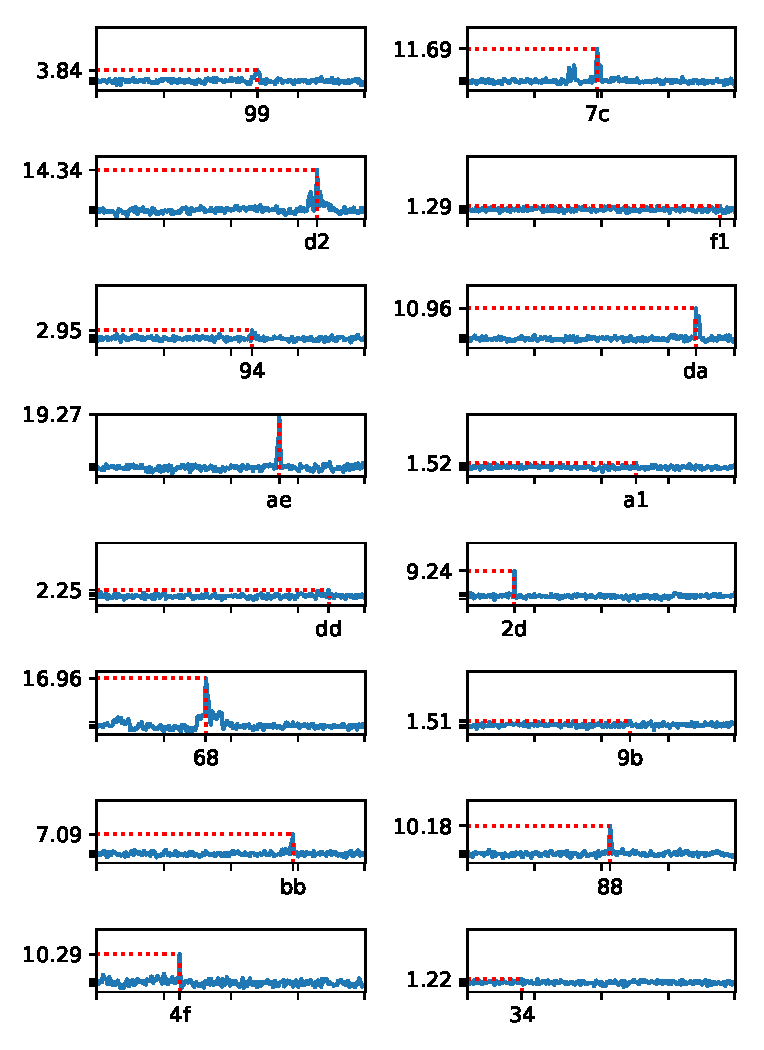
\includegraphics{full_tbox_xeon_success.pdf}
	\caption[Custom T-box on Windows in the lab]{Testing in the InfoSec lab at FIT CTU. A brute-force attack would break the rest of $k$ in less than a day. \\
	CPU: Intel Xeon E3-1245 v6, OS: Windows 10, Impl.: custom T-box, $N_k = 10$, $N_b = 2^{23}$, $N_c = 15$}
\end{figure}

\begin{figure}
	\centering
	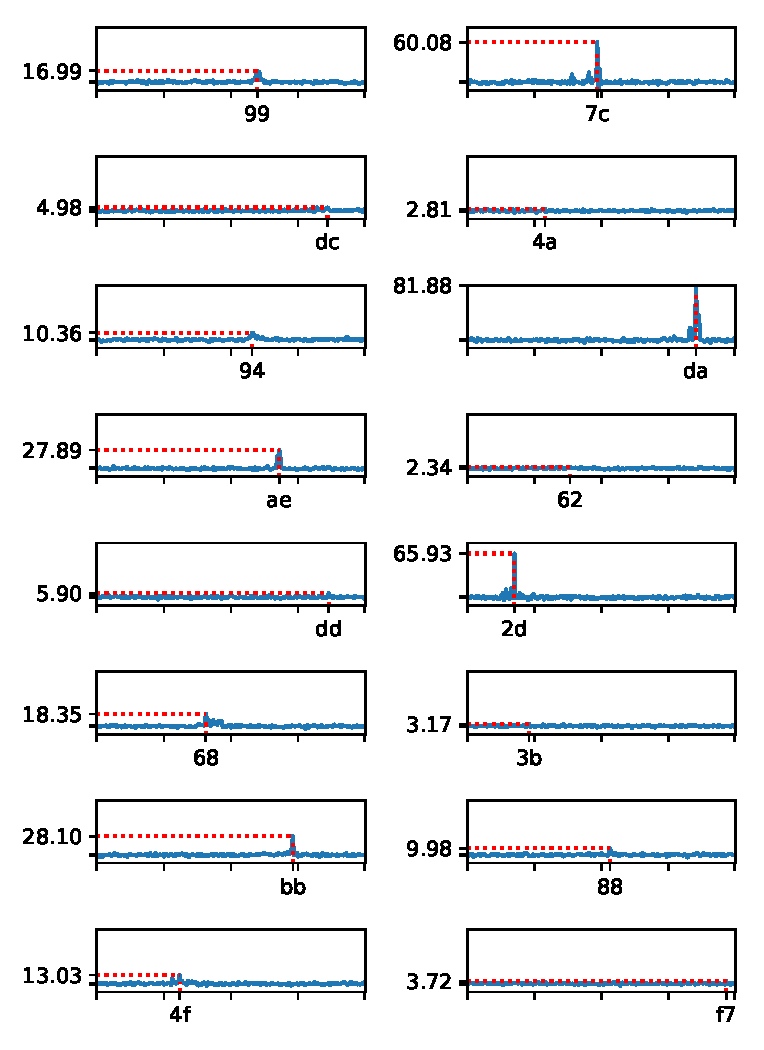
\includegraphics{full_tbox_desktop_success.pdf}
	\caption[Custom T-box on Windows using Core i5-8600K CPU]{Brute-force attack took 2 seconds after 25 runs of the core \\
	CPU: Intel Core i5-8600K, OS: Windows 10, Impl.: custom T-box, $N_k = 10$, $N_b = 2^{23}$, $N_c = 25$}
\end{figure}
% Linux runs
\begin{figure}
	\centering
	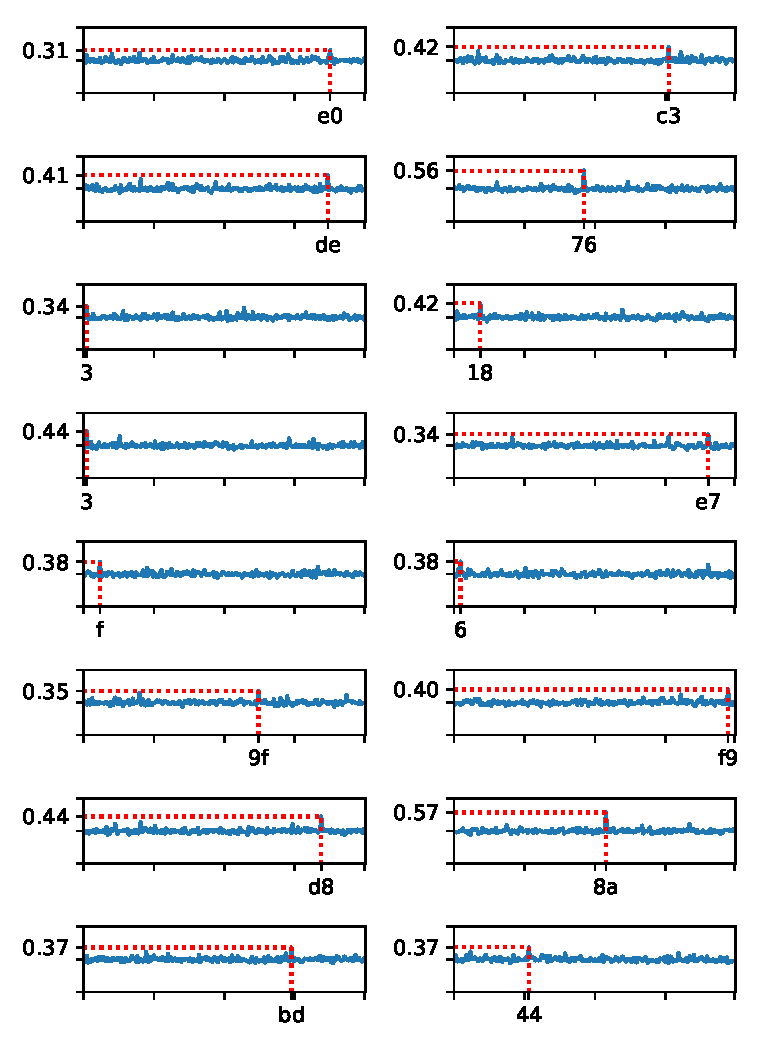
\includegraphics{full_nofilter_laptop.pdf}
	\caption[Unfiltered attack failure]{Removing the cutoff yields noisy and bad data (notice the misleading spikes). \\
	CPU: Intel Core i5-6300HQ, OS: Linux, Impl.: custom T-box, $N_k = 10$, $N_b = 2^{23}$, $N_c = 1$}
\end{figure}

\begin{figure}
	\centering
	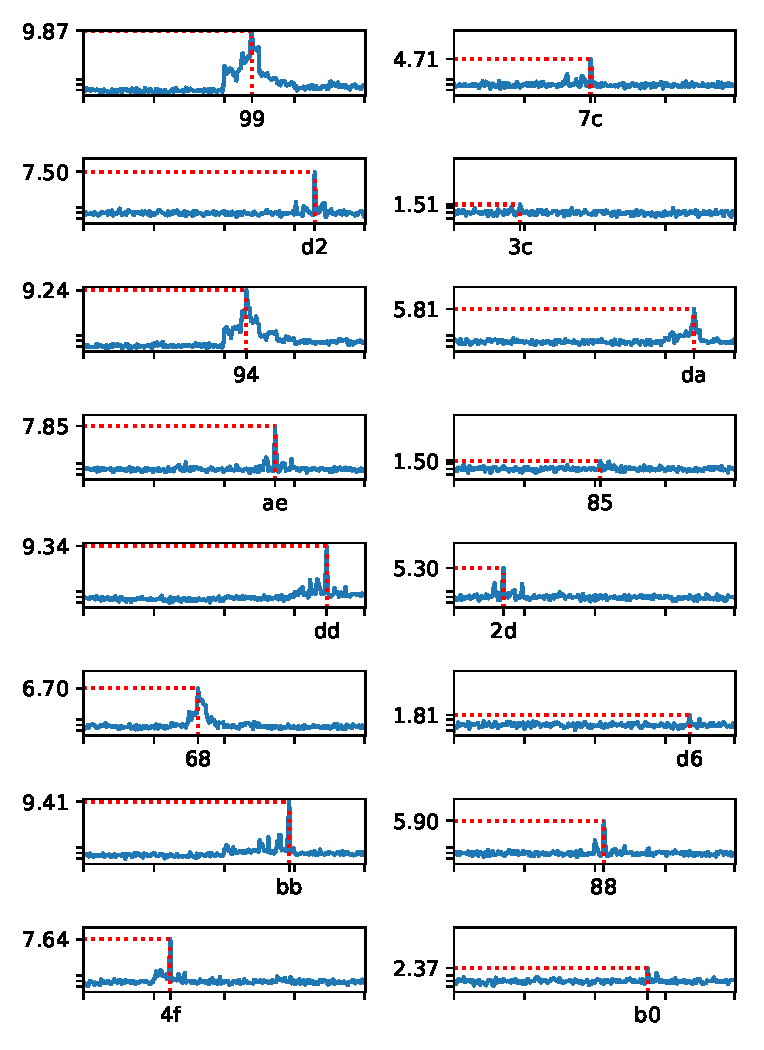
\includegraphics{full_openssl_success.pdf}
	\caption[A successful attack against OpenSSL fallback implementation]{After 25 runs of the core, a brute-force attack would take less than a second. \\
	CPU: Intel Core i5-6300HQ, OS: Linux, Impl.: OpenSSL no-asm, $N_k = 1$, $N_b = 2^{23}$, $N_c = 24$}
\end{figure}

\begin{figure}
	\centering
	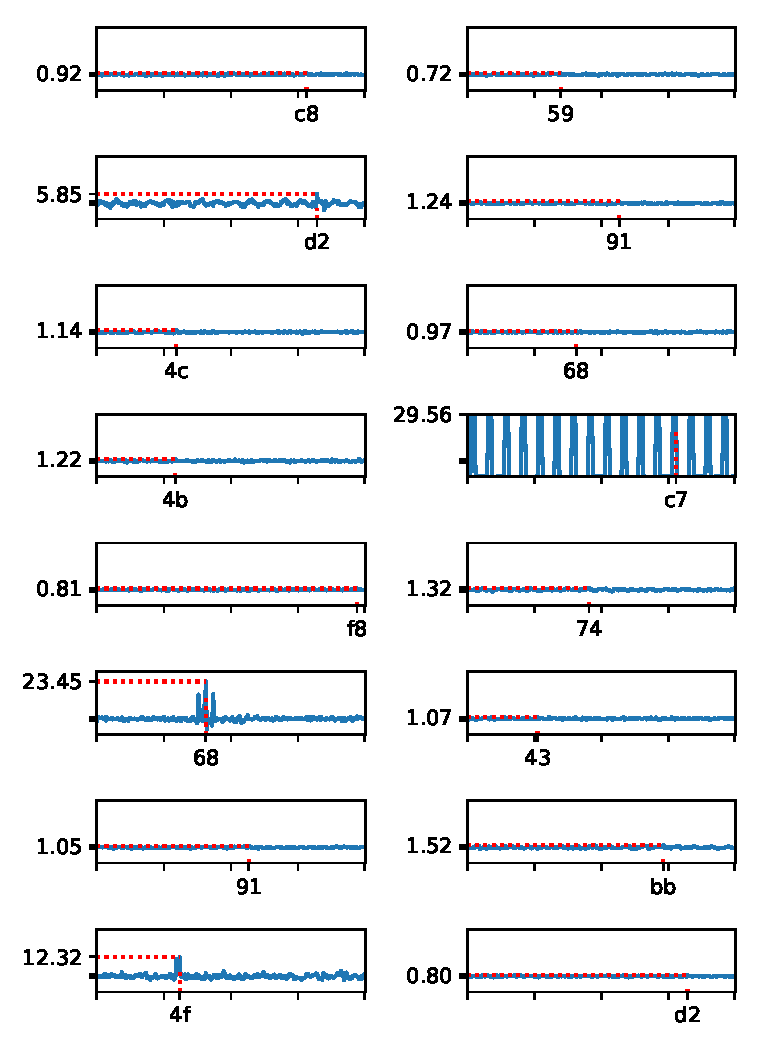
\includegraphics{full_tbox_coreduo.pdf}
	\caption[Custom T-box on Core 2 Duo]{The wave pattern ($k[7]$) appears even with my T-box implementation. \\
	CPU: Intel Core 2 Duo, OS: Linux, Impl.: custom T-box, $N_k = 5$, $N_b = 2^{22}$, $N_c = 5$}
\end{figure}

\end{document}
